\subsection{Tutorial: From Gradient Descent to Optimizer Families}
\label{sec:opt-tutorial}

The rest of this appendix is a reference: one entry per optimizer, with its
update rule, pseudocode, and memory profile. This subsection is the on-ramp.
It introduces the five ideas that every entry reuses---the loss surface, the
gradient, the step size, the batch, and the two statistics that later methods
add---and then compares the families as families, without deriving any single
method. A reader who finishes it should be able to open any of the following
sections and recognise which of the five ideas it is modifying.

\subsubsection{One problem, many recipes}
\label{sec:opt-tutorial-problem}

Training a neural network is an optimization problem wrapped in bookkeeping.
Write $\theta$ for the vector of all trainable numbers (weights and biases,
tens of millions for a small transformer), $L(\theta)$ for the loss, and
$f(\theta)$ for the objective actually minimised, usually $L$ plus a
regulariser. The architecture only decides \emph{which} surface $L$ is: the
number of layers, the attention pattern, the normalisation, the activation.
The optimizer decides \emph{how the walk over that surface proceeds}. Every
optimizer in this appendix can be written as one line,
\begin{equation}
\theta_{t+1} \;=\; \theta_t \;-\; \eta_t\, u_t,
\qquad u_t = u\!\left(g_t, g_{t-1}, \dots,\, \theta_t\right),
\label{eq:opt-tut-generic}
\end{equation}
where $g_t=\nabla f(\theta_t)$ is the gradient and $u_t$ is a direction built
from the current gradient and, possibly, a small amount of remembered state.
Gradient descent takes $u_t=g_t$. Momentum takes $u_t$ to be a decaying
average of past gradients. Adaptive methods divide $u_t$ coordinate by
coordinate. Second-order methods rotate it with a curvature estimate.
Orthogonality methods reshape it as a matrix. Nothing else changes: the sign
in front of $\eta_t$ is always negative, because the gradient points uphill.

The usual picture is a hiker descending a mountain in fog~\citep{ibm_sgd_2025}.
The hiker feels the slope underfoot but cannot see the valley, so the strategy
reduces to three questions: how confident is the slope reading (one example or
a thousand?), how long is the stride, and how much memory of the terrain is
worth carrying. Figure~\ref{fig:opt-tut-flow} turns those questions into the
map of the families that follow.

\begin{figure}[H]
\centering
\fitfigure{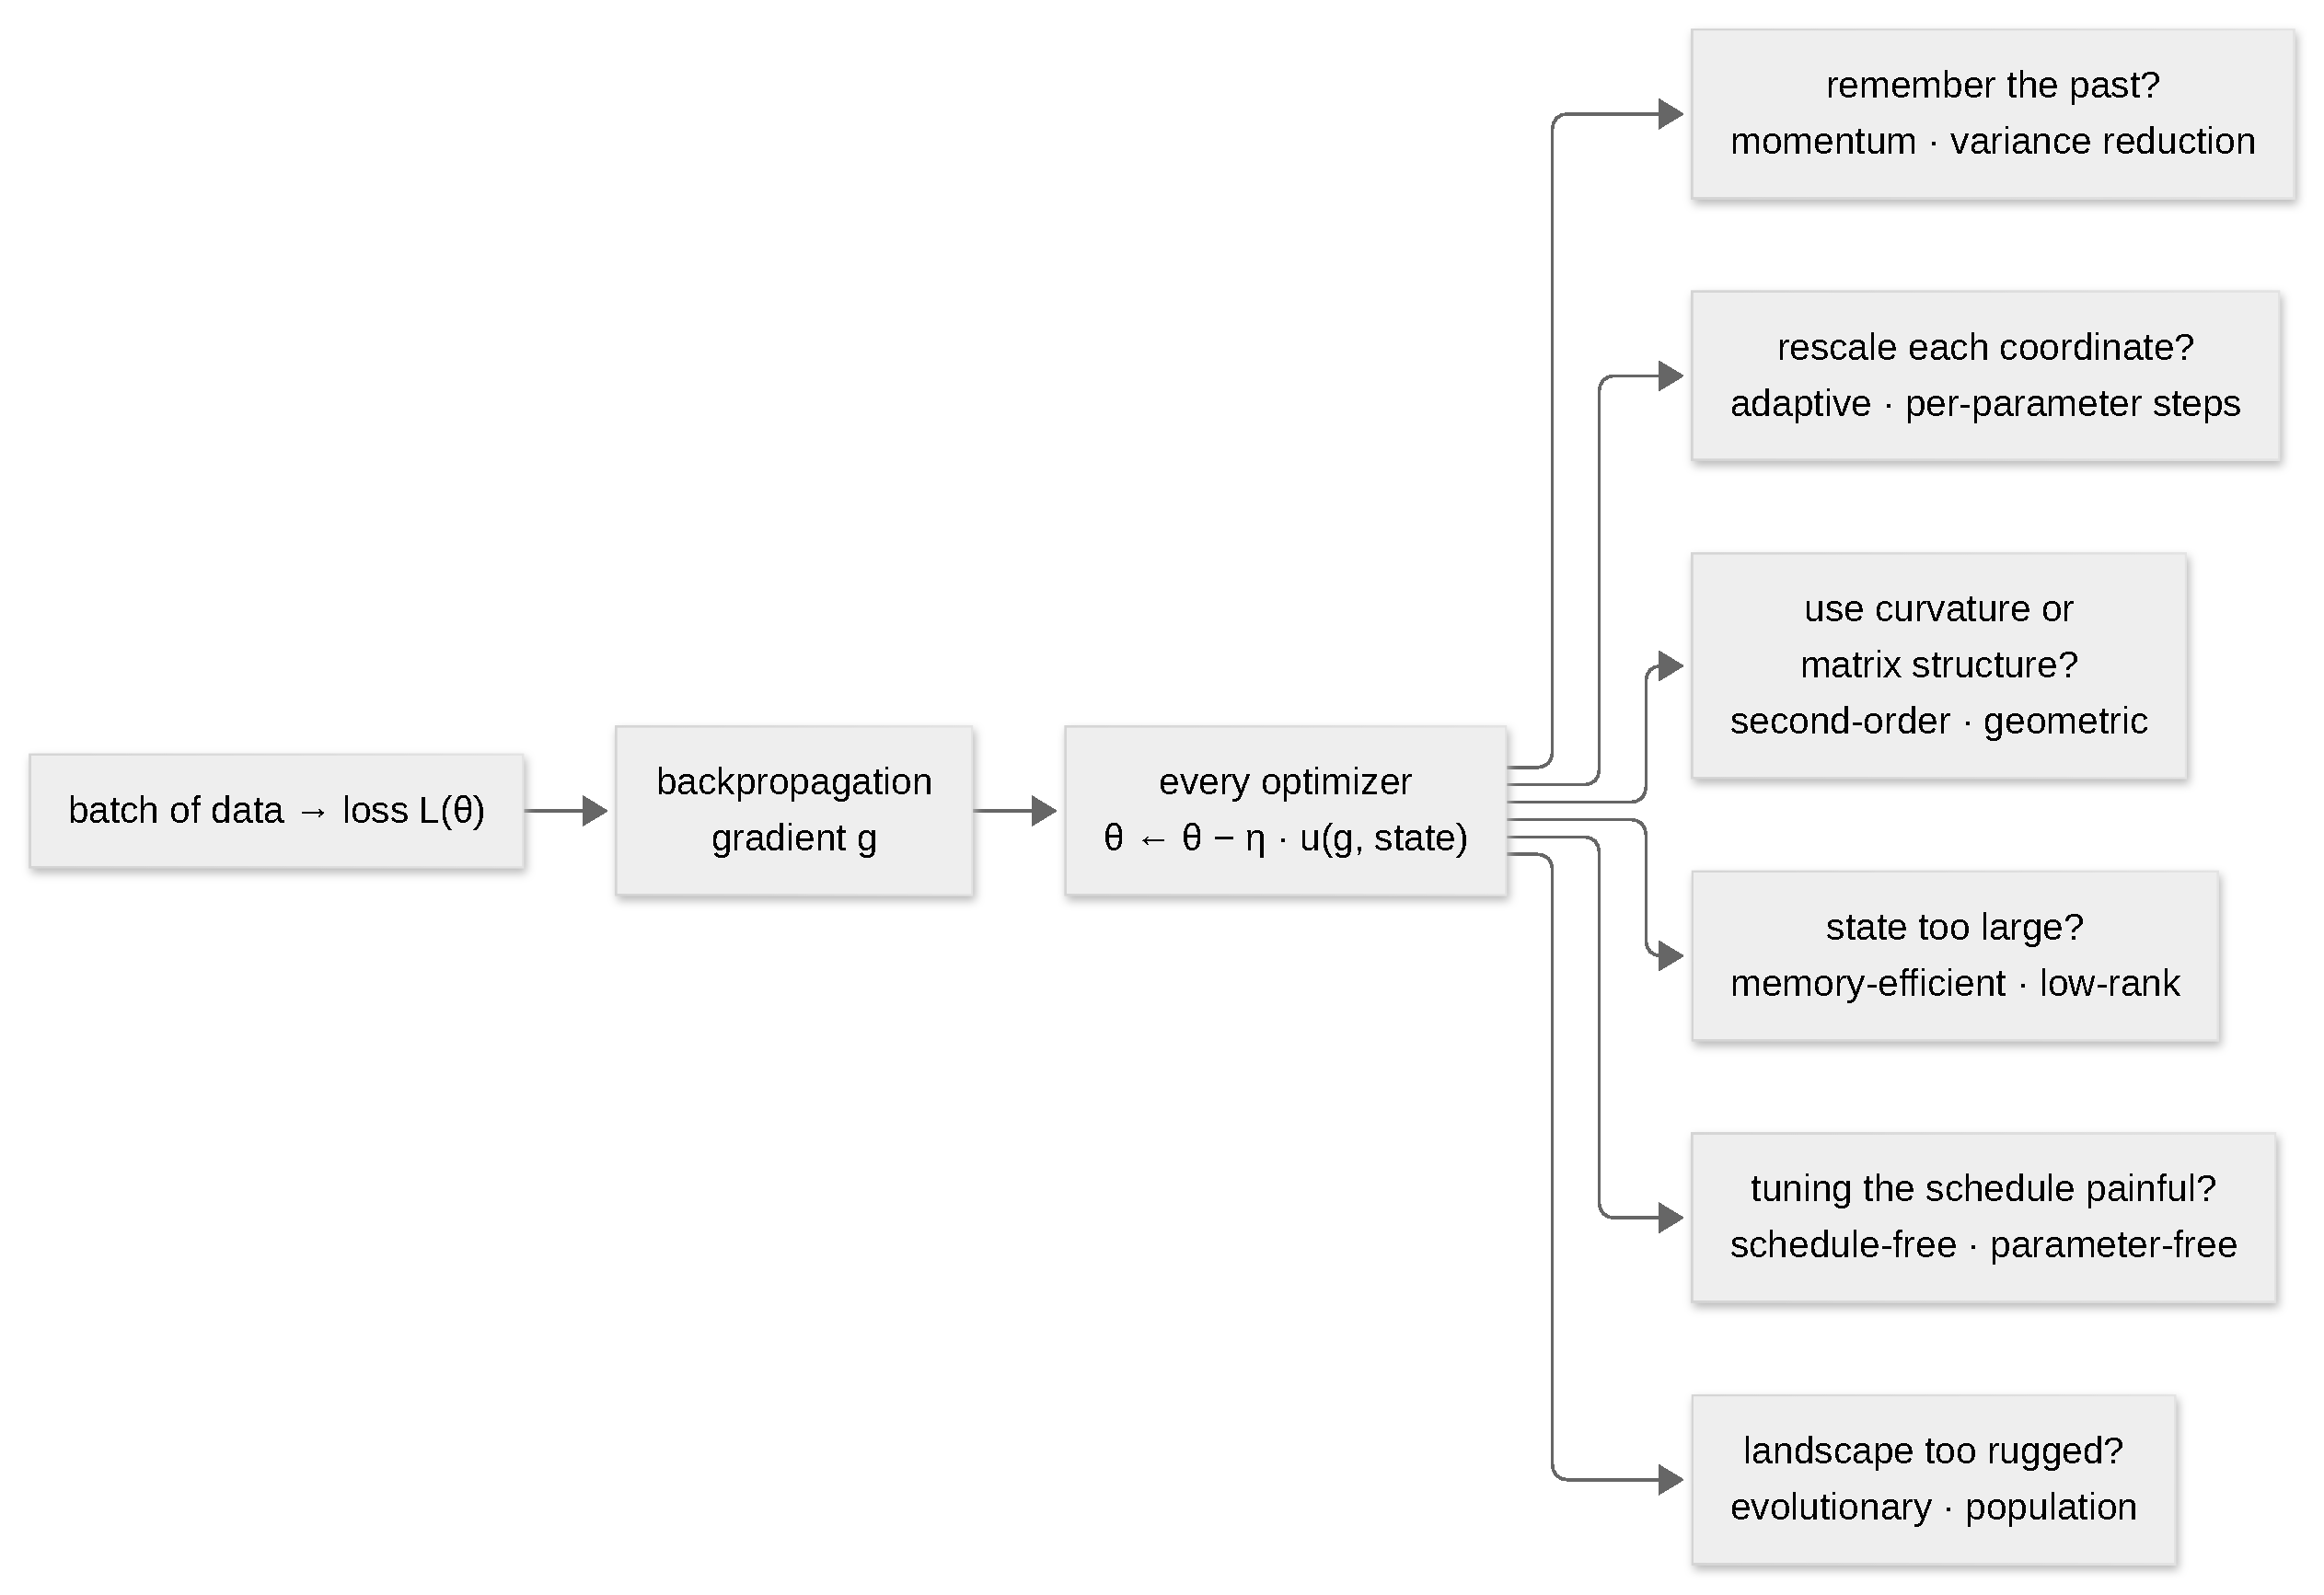
\includegraphics{figures/optimizer-tutorial-flow.pdf}}
\caption{The whole appendix on one page. Data produces a loss, backpropagation
turns the loss into a gradient, and every optimizer applies the same update
rule with a different answer to one of six questions. The questions are
independent, which is why methods can be combined; they are also the only
dimension on which the families in
Section~\ref{sec:annex-optimizers} differ.}
\label{fig:opt-tut-flow}
\end{figure}

\subsubsection{Gradient descent: walk downhill}
\label{sec:opt-tutorial-gd}

For a single weight $w$, the derivative $f'(w)$ is the slope: positive means
the loss grows to the right, so the useful move is to the left. In several
dimensions the gradient $\nabla f$ collects all partial derivatives and points
in the direction of steepest increase; its negative is the direction of
steepest decrease. Taking a step of length $\eta$ along it gives
\begin{equation}
\theta_{t+1} = \theta_t - \eta\,\nabla f(\theta_t),
\label{eq:opt-tut-gd}
\end{equation}
the oldest algorithm in the appendix, usually credited to Cauchy in the
nineteenth century and analysed by Curry in 1944~\citep{ghojogh_ghodsi_2024}. The scalar $\eta>0$ is the
\emph{learning rate} or step size, and it is the only tunable number.

Two facts explain almost everything that follows. First, the step size has a
hard ceiling. If the gradient changes at most $L$ times faster than the
parameters change (the gradient is \emph{$L$-smooth}), then
\eqref{eq:opt-tut-gd} decreases the loss for $\eta<2/L$ and diverges beyond
it; the safe monotone choice is $\eta\le 1/L$~\citep{ghojogh_ghodsi_2024}.
Second, contour lines of a quadratic loss are ellipses whose axes have very
different lengths, and the negative gradient is perpendicular to the contour
but generally does \emph{not} point at the minimum---except when the ellipses
are circles~\citep{hinton_csc321_2012}. The walk therefore zig-zags across the
steep direction while creeping along the flat one.
Figure~\ref{fig:opt-tut-gd} shows the three regimes on the same bowl, and
Figure~\ref{fig:opt-tut-lr} shows what they look like as a loss curve.

\begin{figure}[H]
\centering
\fitfigure{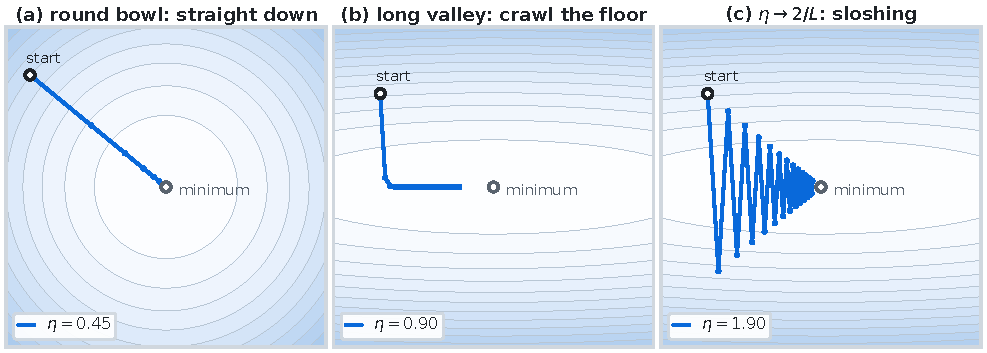
\includegraphics{figures/optimizers/tutorial/tut-gd-landscape.pdf}}
\caption{Gradient descent on a quadratic bowl, same start, 26 steps.
(a) An isotropic bowl: the gradient aims at the minimum and the walk is a
straight line. (b) A valley whose curvature differs by a factor of twenty
between its axes: the steep direction is solved in a few steps, then the walk
crawls along the floor because the same $\eta$ is far too small there.
(c) The same valley with $\eta$ pushed towards the stability limit $2/L$: the
steep direction now alternates sign and the path sloshes. One global step
size cannot serve both directions---the observation that motivates every
per-coordinate method in this appendix~\citep{hinton_csc321_2012}.}
\label{fig:opt-tut-gd}
\end{figure}

\begin{figure}[H]
\centering
\fitfigure{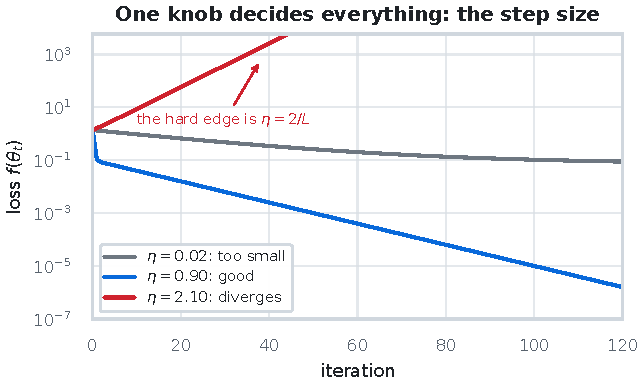
\includegraphics{figures/optimizers/tutorial/tut-learning-rate.pdf}}
\caption{The same valley, one knob. With $\eta$ far below $1/L$ the loss
barely moves; at $\eta\approx1/L$ it falls geometrically; past $\eta=2/L$ every
iteration multiplies the error by a factor larger than one and the run
diverges. The two rates that matter---$1/L$ for monotone decrease and $2/L$
for stability---depend on the curvature, which is exactly what a practitioner
does not know in advance.}
\label{fig:opt-tut-lr}
\end{figure}

When the curvature is unknown, the classical remedy is a \emph{line search}:
try $\eta=1$, halve it until the loss actually decreases, and repeat
\citep{ghojogh_ghodsi_2024}. Deep learning rarely does this, because every
trial costs a full pass over the data; it schedules $\eta$ by hand instead.
Theory supplies the pace: for a convex $L$-smooth objective, gradient descent
reaches $f(\theta_t)-f^\star\le 2L\|\theta_0-\theta^\star\|^2/(t+1)$, that is,
$O(1/t)$~\citep{ghojogh_ghodsi_2024}. Halving the distance to the optimum costs
a doubling of iterations---a fair summary of why first-order methods need so
many steps.

\subsubsection{Where the gradient comes from: backpropagation}
\label{sec:opt-tutorial-backprop}

Nothing above said how to obtain $g_t$. For a network with millions of
weights there is no formula to differentiate by hand, and finite differences
would cost one forward pass per parameter. Backpropagation computes all
partial derivatives in a single backward sweep, using only the chain rule.

In a feed-forward network each layer alternates an affine map and an
activation, $a^{(\ell)}=W^{(\ell)}z^{(\ell-1)}+b^{(\ell)}$ and
$z^{(\ell)}=\sigma(a^{(\ell)})$. The forward pass stores every $a$ and $z$. The
backward pass then propagates one number per neuron,
$\delta^{(\ell)}=\partial e/\partial a^{(\ell)}$, from the loss towards the
input,
\begin{equation}
\delta^{(L)} = \frac{\partial e}{\partial z^{(L)}}\odot\sigma'(a^{(L)}),
\qquad
\delta^{(\ell)} = \sigma'(a^{(\ell)})\odot
\left(W^{(\ell+1)\top}\delta^{(\ell+1)}\right),
\qquad
\frac{\partial e}{\partial W^{(\ell)}} = \delta^{(\ell)}\,z^{(\ell-1)\top},
\label{eq:opt-tut-backprop}
\end{equation}
where $\odot$ is the element-wise product. The gradient of a weight is
therefore the product of a backward number and a forward number---the two
quantities drawn in Figure~\ref{fig:opt-tut-backprop}. The recursion is
linear in the layer index, so the whole sweep costs about the same as one
extra forward pass, roughly twice the forward cost per step, and it must keep
the activations of every layer in memory until they are used
\citep{ghojogh_ghodsi_2024,rumelhart1986learning}.

\begin{figure}[H]
\centering
\fitfigure{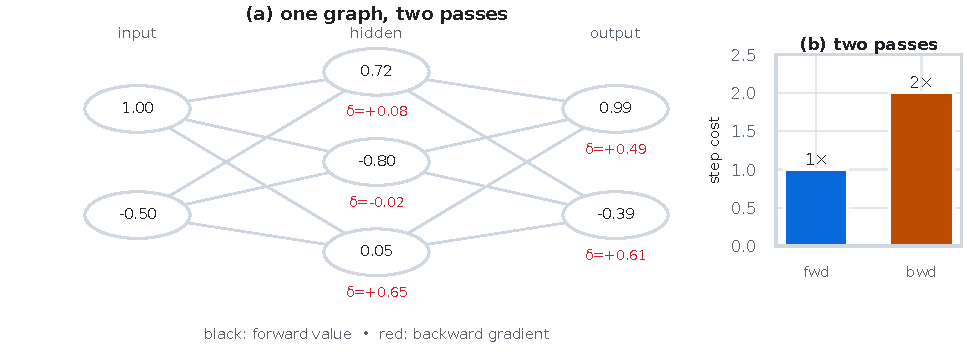
\includegraphics{figures/optimizers/tutorial/tut-backprop.pdf}}
\caption{One training step on a two-hidden-layer network with exact values.
Black numbers are the forward activations $z$; red numbers are the backward
quantities $\delta=\partial e/\partial a$. Every weight gradient is the
product of one red and one black number (equation~\ref{eq:opt-tut-backprop}),
so one backward sweep yields all of them at once. Panel (b): the backward pass
costs about twice the forward pass and keeps the activations alive, which is
why optimizer memory is not the only memory bill in training.}
\label{fig:opt-tut-backprop}
\end{figure}

\begin{algorithm}[H]
\caption{Backpropagation: the gradient factory}
\label{alg:opt-tut-backprop}
\begin{algorithmic}[1]
\Require Input $x$, target $y$, weights $\{W^{(\ell)},b^{(\ell)}\}_{\ell=1}^{L}$
\Ensure Gradients $\{\partial e/\partial W^{(\ell)}\}_{\ell=1}^{L}$
\State Forward: $z^{(0)}\gets x$; \textbf{for} $\ell=1,\dots,L$ \textbf{do} $a^{(\ell)}\gets W^{(\ell)}z^{(\ell-1)}+b^{(\ell)}$, $z^{(\ell)}\gets\sigma(a^{(\ell)})$
\State Loss: $e \gets \ell(z^{(L)}, y)$
\State $\delta^{(L)} \gets \partial e/\partial z^{(L)} \odot \sigma'(a^{(L)})$
\For{$\ell = L, L-1, \dots, 1$}
    \State $\partial e/\partial W^{(\ell)} \gets \delta^{(\ell)} z^{(\ell-1)\top}$
    \State $\partial e/\partial b^{(\ell)} \gets \delta^{(\ell)}$
    \State $\delta^{(\ell-1)} \gets \sigma'(a^{(\ell-1)})\odot\left(W^{(\ell)\top}\delta^{(\ell)}\right)$
\EndFor
\State \Return all weight gradients
\end{algorithmic}
\end{algorithm}

The important consequence for this appendix is that backpropagation is not an
optimizer. It is a gradient factory, and it always returns the exact gradient
of whatever batch it was given. Every difference between the families that
follow lives after the factory, in how $u_t$ in
\eqref{eq:opt-tut-generic} is formed.

\subsubsection{Stochastic and mini-batch gradient descent}
\label{sec:opt-tutorial-sgd}

With $n$ examples the loss is an average, $f(\theta)=\frac1n\sum_i f_i(\theta)$,
so the exact gradient is an average of $n$ per-example gradients and one step
costs $n$ backward passes. For a dataset of a billion tokens that is
unaffordable, and it is also wasteful: neighbouring examples usually say
almost the same thing about the parameters.

Stochastic gradient descent, in the line of the Robbins--Monro stochastic
approximation~\citep{robbins_monro_1951}, replaces the average by one term,
$\hat g_t=\nabla f_{i_t}(\theta_t)$ with $i_t$ drawn uniformly, giving
\begin{equation}
\theta_{t+1} = \theta_t - \eta_t\,\nabla f_{i_t}(\theta_t).
\label{eq:opt-tut-sgd}
\end{equation}
The estimate is unbiased, $\mathbb{E}[\hat g_t]=g_t$, so on average it points
the right way; its error falls as $\sigma/\sqrt{b}$ when a batch of $b$
examples is used instead of one
\citep{ghojogh_ghodsi_2024,bottou_2010}. Modern libraries call this
\emph{mini-batch} method ``SGD'' and almost never use $b=1$: one pass over the
data (an \emph{epoch}) then contains $\lfloor n/b\rfloor$ updates rather than
one~\citep{ibm_sgd_2025,ghojogh_ghodsi_2024}. Figure~\ref{fig:opt-tut-noise}
shows both faces of the trade: with the same number of steps and the same step
size, small batches wander, and the noise they inject is precisely the
quantity that shrinks as $1/\sqrt{b}$.

\begin{figure}[H]
\centering
\fitfigure{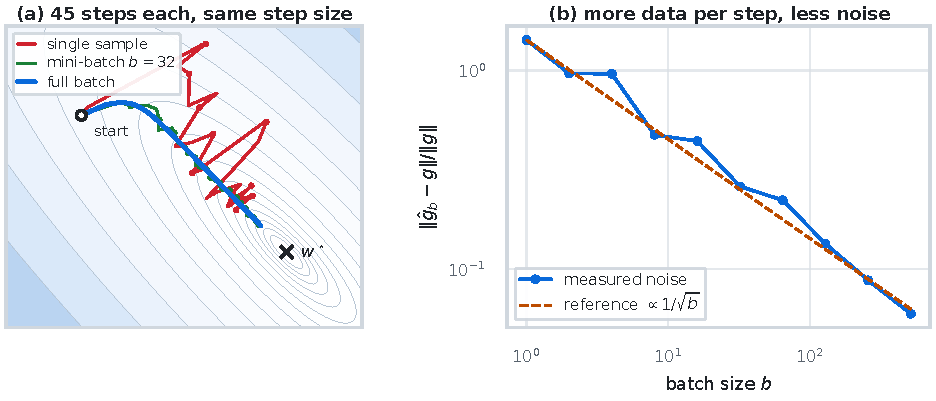
\includegraphics{figures/optimizers/tutorial/tut-batch-noise.pdf}}
\caption{(a) A real least-squares surface in two weights (correlated features,
so the valley is genuine), with 45 steps from the same start and the same step
size. The full batch descends smoothly; a mini-batch of 32 tracks it with a
visible wobble; single-sample gradients never settle. (b) Relative error of
the batch gradient against the full gradient, measured on the same data: the
measured points follow the $1/\sqrt{b}$ law, the noise is halved by
quadrupling the batch.}
\label{fig:opt-tut-noise}
\end{figure}

Noise is not only a cost. Because each step is a random approximation, the
iterate can leave a shallow basin or slide across a saddle that a full-batch
method would treat as a stopping point~\citep{ibm_sgd_2025}. The price appears
in the rate. For a convex $L$-smooth objective, SGD with $\eta_t\propto1/\sqrt
t$ satisfies $f(\theta_t)-f^\star=O(\log t/\sqrt t)$, and with a constant step
it converges to a neighbourhood of size $O(\eta)$ and then
stalls~\citep{ghojogh_ghodsi_2024}. Full-batch gradient descent is therefore
more accurate per iteration and much slower per iteration; SGD is the
opposite. Figure~\ref{fig:opt-tut-rates} puts the two statements on the same
axes, once per iteration and once per unit of wall-clock, which is the
comparison that actually matters when a step costs $n/b$ times less.

\begin{figure}[H]
\centering
\fitfigure{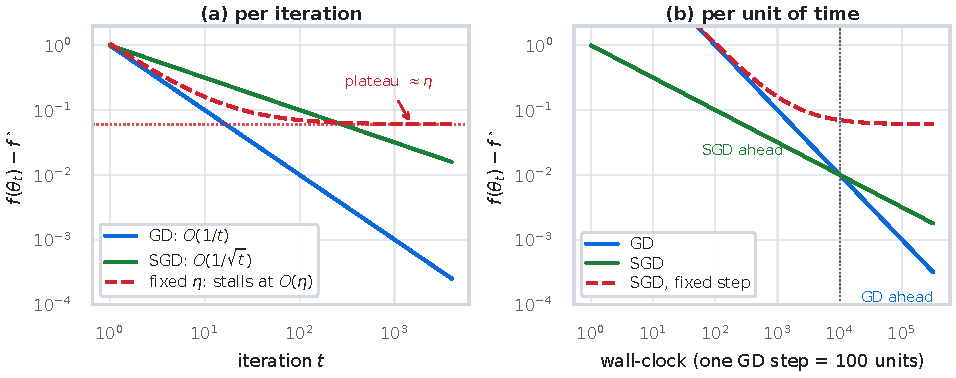
\includegraphics{figures/optimizers/tutorial/tut-convergence.pdf}}
\caption{(a) Per iteration, gradient descent decays as $O(1/t)$ while SGD
decays as $O(1/\sqrt t)$ and, with a fixed step, flattens at a plateau of
height $O(\eta)$~\citep{ghojogh_ghodsi_2024}. The plateau is the reason every
practical recipe eventually reduces $\eta$. (b) The same curves against
wall-clock, with one full-batch step costing a hundred mini-batch steps: SGD
is ahead for most of the run and gradient descent only wins once the plateau
binds. Curves are schematic, with constants chosen for legibility.}
\label{fig:opt-tut-rates}
\end{figure}

\subsubsection{Two knobs that every later method turns}
\label{sec:opt-tutorial-knobs}

Everything after this point is a refinement of two observations about
equation~\eqref{eq:opt-tut-gd}, and it is worth separating them before meeting
the families.

\paragraph{Memory of the past.} A ball rolling down the same valley keeps its
velocity: it accumulates speed along a consistent slope and cancels the
oscillation when the slope keeps changing sign. Momentum implements exactly
that, replacing the gradient by a decaying sum of gradients,
\begin{equation}
v_t = \beta\,v_{t-1} - \eta\,g_t,
\qquad
\theta_{t+1} = \theta_t + v_t,
\label{eq:opt-tut-momentum}
\end{equation}
with $\beta\in[0,1)$ the decay. The effective step is $\eta/(1-\beta)$ along a
steady direction, which is how a small $\eta$ can still move quickly. Nesterov
momentum makes the same move but reads the gradient at the position the
velocity is heading towards, so the correction arrives before the overshoot
does~\citep{hinton_csc321_2012,sutskever2013importance}. Figure
\ref{fig:opt-tut-momentum} shows the composition of the two terms and its
effect on the valley.

\begin{figure}[H]
\centering
\fitfigure{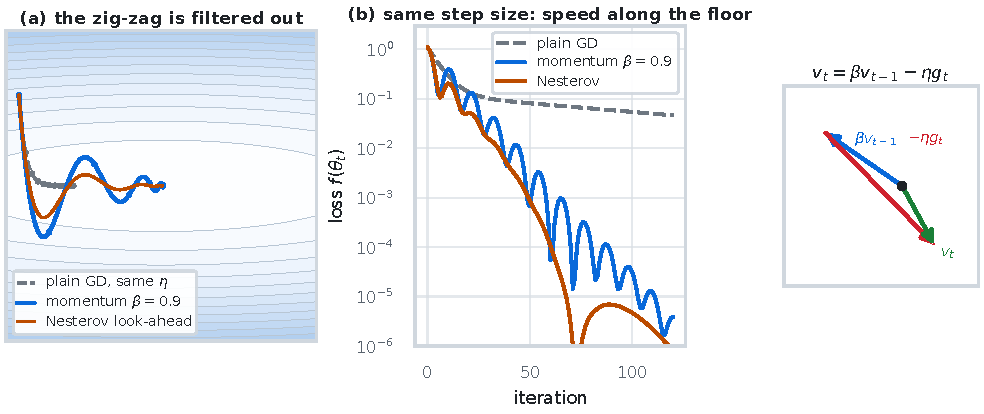
\includegraphics{figures/optimizers/tutorial/tut-momentum.pdf}}
\caption{Momentum as memory. (a) On the valley of
Figure~\ref{fig:opt-tut-gd}(b), with the same step size, plain gradient
descent still crawls along the floor after 120 steps while momentum and its
Nesterov variant reach the minimum. (b) The same run as a loss curve: the
remembered direction buys roughly an order of magnitude. (c) The update is the
head-to-tail sum of the decayed velocity (blue) and the fresh gradient step
(red); the result (green) is smoother than either term alone.}
\label{fig:opt-tut-momentum}
\end{figure}

\paragraph{One step size per coordinate.} The second observation is that the
valley of Figure~\ref{fig:opt-tut-gd}(b) has no single good $\eta$: what is
stable along the steep axis is negligible along the flat one. Adaptive
methods keep a running average of squared gradients and divide by its square
root, so a coordinate that has been receiving large gradients gets a smaller
step and a quiet coordinate gets a larger one,
\begin{equation}
s_t = \gamma\,s_{t-1} + (1-\gamma)\,g_t^2,
\qquad
\theta_{t+1} = \theta_t - \eta\,\frac{g_t}{\sqrt{s_t}+\epsilon}.
\label{eq:opt-tut-rms}
\end{equation}
The scheme grew out of rprop, which used only the sign of the gradient, and
its mini-batch version, rmsprop~\citep{hinton_csc321_2012,tieleman_hinton2012};
AdaGrad is the cumulative rather than decaying version~\citep{duchi_adagrad_2011}.
Figure~\ref{fig:opt-tut-adaptive} shows the effect: the two axes of the valley
receive comparable displacements, at the cost of a per-coordinate state and a
step that no longer shrinks on its own---the residual jitter of size
$\approx\eta$ around the minimum is what later motivates decaying or
schedule-free step sizes.

\begin{figure}[H]
\centering
\fitfigure{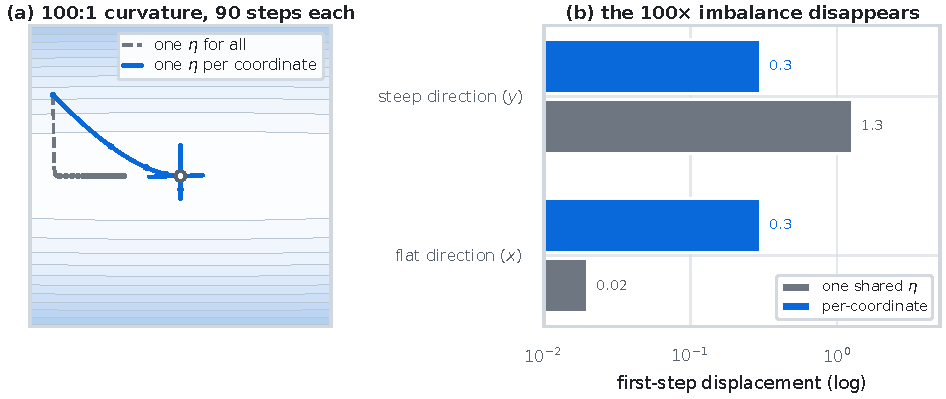
\includegraphics{figures/optimizers/tutorial/tut-adaptive.pdf}}
\caption{One step size per coordinate. (a) On a valley with a hundred-to-one
curvature ratio, a shared step size either overshoots the steep axis or
ignores the flat one; normalising each coordinate by the root-mean-square of
its recent gradients reaches the basin and jitters around it. (b) First-step
displacement per coordinate, on a logarithmic axis: the shared step size
produces a factor of sixty between the axes, the normalised one produces
none.}
\label{fig:opt-tut-adaptive}
\end{figure}

The two knobs compose, and their composition is the reason AdamW is the
default in practice: a first moment for direction, a second moment for scale,
a bias correction for the empty first steps, and a decoupled weight decay for
regularisation~\citep{kingma_adam_2014}. Nothing in
equations~\eqref{eq:opt-tut-momentum} and~\eqref{eq:opt-tut-rms} is specific to
transformers; what differs across the families is which statistics are kept,
how they are combined, and how many bytes per parameter that costs. A compact
survey of the resulting zoo is given by \citet{ruder_2016}.

\subsubsection{How the families differ}
\label{sec:opt-tutorial-families}

The appendix that follows contains thirty-eight methods, which is too many to
hold in mind at once. They are easier to remember as eight families, each
answering one of the questions in Figure~\ref{fig:opt-tut-flow} and each
distinguished by what it remembers and what it pays.

\begin{itemize}[leftmargin=*]
\item \textbf{First-order baselines} (SGD with momentum, AdamW, RAdam) keep one
or two statistics per parameter and assume the landscape is smooth enough for
a locally linear model. They are the reference against which everything else
is measured.
\item \textbf{Momentum and variance reduction} (Adan, ADOPT, AdEMAMix, MARS,
Cautious AdamW) keep more than two buffers, or a gradient difference, to
reduce the variance of the update itself. They buy stability and speed at the
cost of memory and of a second gradient evaluation or a longer history.
\item \textbf{Memory-efficient and low-rank} (Adafactor, GaLore, APOLLO, Lion,
AdamPM) accept a worse estimate of the second moment---a factored one, a
projected one, or none---precisely to shrink the state. Lion goes as far as
keeping only the sign of the update.
\item \textbf{Schedule-free and parameter-free} (Schedule-Free AdamW,
Prodigy, LAMB for large batches) move the burden of choosing $\eta_t$ from the
practitioner to the algorithm, usually by averaging iterates or by estimating
the step from the loss itself.
\item \textbf{Curvature and second-order} (Sophia, Shampoo, SOAP) estimate how
the gradient changes, not just its size, and precondition the step with that
estimate. They converge in fewer iterations and cost more per iteration.
\item \textbf{Geometric and orthogonality} (Muon, Turbo-Muon, AF-Muon, ROOT,
NorMuon, Dion3) treat a weight matrix as a matrix: they orthogonalise or
otherwise whiten the update so that all singular directions move at the same
rate, which is a cheap surrogate for curvature on matrix-shaped parameters.
\item \textbf{Adaptivity-tunable} (Anon) keeps the standard state but adapts
its own coefficients, so the amount of adaptivity is a hyperparameter rather
than a fixed design choice.
\item \textbf{Evolutionary and population} (EvE, EA4LLM) do not follow a
gradient at all: they sample perturbations or maintain a population of models,
which is attractive when gradients are noisy, unavailable, or when many
hyperparameters must be tuned at once, and expensive when the model is large.
\end{itemize}

Table~\ref{tab:opt-tut-families} states the same comparison in the two
currencies that decide a real training run: what is stored per parameter and
what each step costs. Figure~\ref{fig:opt-tut-families} turns it into a
fingerprint: reading down a row tells you which ingredients a family uses,
reading across a column tells you which families share one.

\begin{table}[H]
\centering
\caption{The eight families by the question they answer and what they cost.
State is approximate, in floats per parameter; $k$ is a rank or block count,
$P$ a population size. No family is uniformly better: each line is a trade.}
\label{tab:opt-tut-families}
\small
\begin{tabular}{@{}L{3.2cm}L{4.6cm}L{2.6cm}L{4.6cm}@{}}
\toprule
Family & Question answered & State per parameter & Main risk \\
\midrule
First-order baseline & What is the slope? & 0--2 & needs a hand-tuned schedule \\
Momentum, variance reduction & Which way is it going? & 2--3 & more memory and bookkeeping \\
Memory-efficient, low-rank & Can the state be smaller? & $\le1$ & biased second moment \\
Schedule-free, parameter-free & Can $\eta_t$ be chosen for me? & 1 & theory assumes convexity \\
Curvature, second-order & How does the slope change? & $2+2k$ & expensive factorisations \\
Geometric, orthogonality & Is the update well shaped? & 1 & matrices only \\
Adaptivity-tunable & How adaptive is it? & 2 & extra hyperparameters \\
Evolutionary, population & Can we search without gradients? & $P\times$ & prohibitive at scale \\
\bottomrule
\end{tabular}
\end{table}

\begin{figure}[H]
\centering
\fitfigure{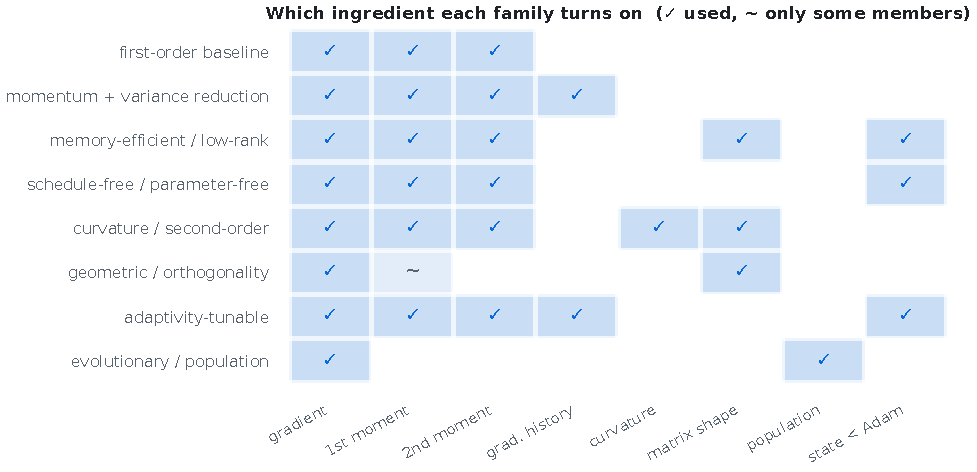
\includegraphics{figures/optimizers/tutorial/tut-families.pdf}}
\caption{A fingerprint of the eight families. A tick marks an ingredient the
family uses, a tilde marks one that only some members use. The first column is
ticked everywhere---every family in this appendix is a gradient method except
the last---and the remaining columns are the actual axes of variation:
direction memory, per-coordinate scale, curvature, matrix structure,
population, and a state smaller than Adam's. The map is deliberately coarse;
the entries that follow give the exact rules.}
\label{fig:opt-tut-families}
\end{figure}

Algorithm~\ref{alg:opt-tut-generic} makes the comparison operational: the
families differ only in which slots they fill. Reading it side by side with
Table~\ref{tab:opt-tut-knobs} is enough to place any method from the rest of
the appendix without memorising its algebra.

\begin{algorithm}[H]
\caption{Any optimizer in this appendix, with the family-specific slots left open}
\label{alg:opt-tut-generic}
\begin{algorithmic}[1]
\Require Parameters $\theta_0$, learning rate $\eta$, slots
$\mathcal{S}$ (state), $\mathcal{D}$ (direction), $\mathcal{P}$ (preconditioner), $\mathcal{T}$ (step rule)
\Ensure Updated parameters $\theta_T$
\State Initialize the state required by $\mathcal{S}$
\For{$t = 1, 2, \ldots, T$}
    \State Sample a batch $\mathcal{B}_t$ and compute $g_t\gets\nabla f_{\mathcal{B}_t}(\theta_{t-1})$ \Comment{backpropagation}
    \State Update the state: $\mathcal{S}\gets\textsc{Update}(\mathcal{S}, g_t, \theta_{t-1})$ \Comment{1st/2nd moment, curvature, population}
    \State Form the direction $u_t\gets\mathcal{D}(g_t,\mathcal{S})$ \Comment{raw gradient, momentum, sign, orthogonalised}
    \State Apply the preconditioner $u_t\gets\mathcal{P}(u_t,\mathcal{S})$ \Comment{per-coordinate scaling, factorised or full}
    \State Choose the step $\eta_t\gets\mathcal{T}(\eta, t, \mathcal{S})$ \Comment{constant, schedule, implicit, self-tuned}
    \State $\theta_t\gets\theta_{t-1}-\eta_t\,u_t$ \Comment{optionally after decoupled weight decay}
\EndFor
\State \Return $\theta_T$
\end{algorithmic}
\end{algorithm}

\begin{table}[H]
\centering
\caption{The slots of Algorithm~\ref{alg:opt-tut-generic} and the knob each one
turns. A method is identified by the slots it fills, not by its name.}
\label{tab:opt-tut-knobs}
\small
\begin{tabular}{@{}L{2.4cm}L{4.4cm}L{3.4cm}L{3.6cm}@{}}
\toprule
Slot & What it decides & Knob turned & Seen in \\
\midrule
$\mathcal{B}_t$ & how many examples per step & variance & SGD, mini-batch, full batch \\
$\mathcal{S}$ & what is remembered & state and memory & momentum, Adam, Sophia, Shampoo \\
$\mathcal{D}$ & which direction is followed & smoothing & momentum, Nesterov, sign methods \\
$\mathcal{P}$ & how coordinates are rescaled & conditioning & AdaGrad, RMSProp, Adam, Muon \\
$\mathcal{T}$ & how long the step is & schedule & cosine, warmup, schedule-free, Prodigy \\
decay & how parameters are regularised & generalisation & L2, decoupled weight decay \\
\bottomrule
\end{tabular}
\end{table}

\subsubsection{Reading a loss curve}
\label{sec:opt-tutorial-diagnostics}

The practical value of the five ideas is diagnostic. A single loss curve
already says which of them is wrong, and the answer is usually visible within
a few hundred steps (Figure~\ref{fig:opt-tut-diag}).

\begin{figure}[H]
\centering
\fitfigure{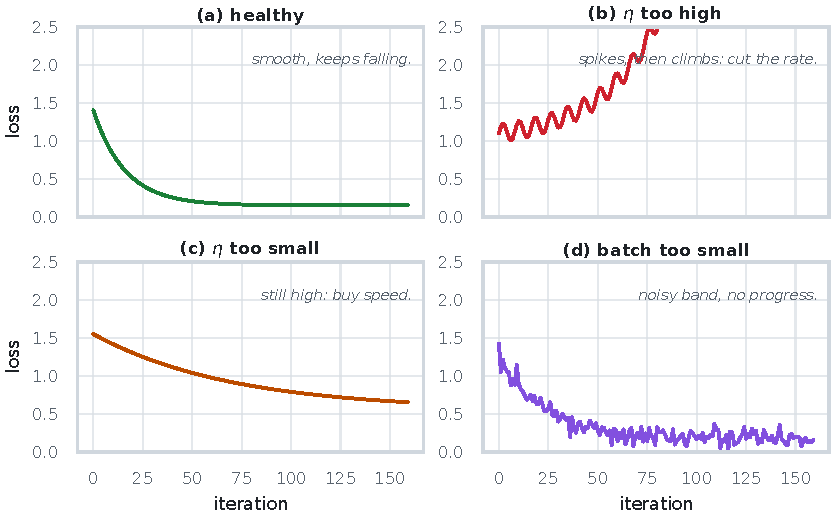
\includegraphics{figures/optimizers/tutorial/tut-loss-diagnostics.pdf}}
\caption{Four loss curves and the sentence each one is saying. A smooth curve
that keeps falling is healthy; spikes followed by a rise mean the step size
crossed $2/L$; a curve that is smooth but far too high means the step size is
far below $1/L$ or the schedule decayed too early; a curve that reaches a
noisy band and stops improving usually means the batch is too small or the
step size has hit its $O(\eta)$ plateau.}
\label{fig:opt-tut-diag}
\end{figure}

Five rules of thumb close the tutorial, all of them consequences of the
figures above rather than of any particular method.
\begin{enumerate}[leftmargin=*]
\item Start from a first-order baseline with both moments (AdamW). It is the
cheapest configuration that survives heterogeneous curvature.
\item If the optimizer state does not fit in memory, change family before
changing hyper parameters: the memory-efficient and low-rank families exist
for exactly that constraint.
\item If tuning the schedule consumes the experiment budget, the schedule-free
and parameter-free families remove the knob instead of tuning it.
\item If most parameters live in matrices (attention and feed-forward
projections), geometric methods exploit a structure that element-wise methods
ignore; if the model is small and the search is over many configurations,
population methods become affordable.
\item Change one slot at a time. Because the families are orthogonal
compositions, a run that changes two of them cannot attribute its result.
\end{enumerate}

The rest of this appendix is the reference behind these statements: one entry
per method, each stating its update rule, its pseudocode, its memory profile,
and the trade it makes.
